\documentclass[conference]{IEEEtran}
\IEEEoverridecommandlockouts

\usepackage{cite}
\usepackage{amsmath,amssymb}
\usepackage{booktabs}
\usepackage{float}
\usepackage{pgfplots}
\usepackage{tikz}
\usepackage{url}
\usepackage{microtype}
\usepackage{balance}
\pgfplotsset{compat=1.18}
\usetikzlibrary{shapes.geometric, arrows.meta, positioning}

\title{
\textbf{Intelligent Credit Risk Assessment:}\\[0.4em]
\large An Agentic AI Approach with RAG and Decision Trees \\
\vspace{0.4cm}
\large Team Members
}

\author{
\IEEEauthorblockN{
Shivansh Bhargava \and 
Devansh Saini \and 
Om Gupta \and 
Sahil Khemnar
}
}

\begin{document}
\maketitle

\begin{abstract}
Traditional credit systems often provide statistical scores without explaining the underlying reasoning. This paper presents an \textbf{Agentic Lending System} that bridges machine learning and explainable AI. We integrate a \textbf{Decision Tree (94.1\% accuracy)} with a \textbf{Retrieval-Augmented Generation (RAG)} framework using FAISS and LangGraph. The system produces both statistical risk probabilities and structured, policy-grounded reports, ensuring ethical compliance and decision transparency.
\end{abstract}

\begin{IEEEkeywords}
Credit Risk, Agentic AI, RAG, LangGraph, Decision Tree
\end{IEEEkeywords}

\vspace{0.2cm}

\section{Introduction}
Financial institutions require both \textit{accuracy} and \textit{transparency} in lending decisions. While Milestone I established a strong statistical foundation, Milestone II extends this into an \textbf{Agentic AI Lending Assistant}.

By leveraging \textbf{Agentic-RAG}, every prediction is contextualized against human-curated ethical guidelines, enabling automated justifications that are professional, interpretable, and audit-ready.

\section{Methodology}

\subsection{Machine Learning Foundation}
The core model uses a \textbf{Decision Tree} due to its inherent interpretability. It mirrors financial decision-making through threshold-based splits and was trained on a \textit{150K-record Credit Risk Benchmark Dataset}.

\subsubsection{Feature Engineering}
To better capture borrower behavior and financial stability, two domain-specific features were introduced:

\begin{enumerate}
\item \textbf{Total Late (Delinquency Score)}
\begin{equation}
\texttt{total\_late} = \sum \text{Delinquency Buckets}
\end{equation}

\item \textbf{Financial Stress Index}
\begin{equation}
\texttt{stress} = \texttt{debt\_ratio} \times \texttt{rev\_util}
\end{equation}
\end{enumerate}

\subsection{Agentic AI Architecture}
The system follows a modular multi-agent workflow orchestrated using \textbf{LangGraph}. Each stage performs a clearly defined role, improving maintainability and interpretability.

\begin{figure}[H]
\centering
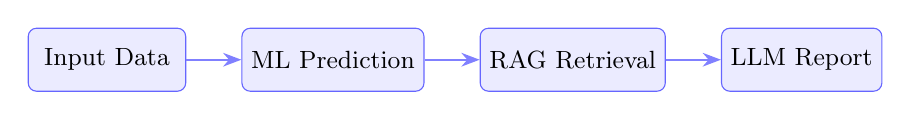
\begin{tikzpicture}[
    node distance=0.7cm,
    block/.style={
        rectangle, rounded corners=3pt,
        draw=blue!60, fill=blue!8,
        minimum height=0.8cm,
        minimum width=2cm,
        align=center,
        font=\small
    },
    arrow/.style={-Stealth, thick, blue!50}
]

\node[block] (input) {Input Data};
\node[block, right=of input] (ml) {ML Prediction};
\node[block, right=of ml] (rag) {RAG Retrieval};
\node[block, right=of rag] (llm) {LLM Report};

\draw[arrow] (input) -- (ml);
\draw[arrow] (ml) -- (rag);
\draw[arrow] (rag) -- (llm);

\end{tikzpicture}
\caption{Agentic Lending Workflow}
\vspace{-0.3cm}
\end{figure}

\subsubsection{Retrieval-Augmented Generation (RAG)}
To ensure factual correctness and prevent hallucinations, a RAG pipeline is implemented:

\begin{itemize}
\item \textbf{Embeddings:} \texttt{all-MiniLM-L6-v2}
\item \textbf{Vector Store:} \textbf{FAISS} for fast similarity search
\end{itemize}

\subsubsection{Agentic Reasoning}
Using \textbf{LangGraph}, the agent processes:
\begin{itemize}
\item Borrower profile
\item ML risk score
\item Retrieved policy rules
\end{itemize}

It generates structured outputs including \textit{Borrower Summary, Risk Analysis, and Mitigation Suggestions}, ensuring decisions remain explainable and policy-compliant.

\section{Implementation and Results}
The system is deployed using \textbf{Streamlit}, with inference powered by the \textbf{Groq API}. A PDF export feature is included for documentation and audit purposes.

\textbf{Performance Metrics:}
\begin{itemize}
\item Accuracy: \textbf{94.1\%}
\item F1-Score: \textbf{0.65}
\end{itemize}

Qualitatively, the RAG agent flags borderline cases as \textit{"Further Review"}, reducing false negatives and improving ethical decision-making. This enhances trust and supports human-in-the-loop validation.

\section{Conclusion}
This work presents a complete \textbf{Agentic Credit Risk Assessment System}. By combining Decision Trees with RAG, the system achieves both statistical robustness and explainable reasoning.

Future work will focus on integrating \textbf{local LLMs} to enhance privacy, reduce dependency on external APIs, and enable fully offline decision-making capabilities.

\balance

\bibliographystyle{IEEEtran}
\begin{thebibliography}{1}
\footnotesize
\bibitem{} Kaggle, ``Credit Risk Dataset,'' 2023.
\bibitem{} LangChain, ``LangGraph Agents,'' 2024.
\bibitem{} J. Johnson, ``FAISS,'' \textit{arXiv:1702.08734}, 2017.
\end{thebibliography}

\end{document}